% !TEX root = ../om_ts_03.tex

\begin{frame} % название фрагмента

\videotitle{Модель ETS: дампированный тренд}

\end{frame}



\begin{frame}{Модель ETS: дампированный тренд}
  \begin{itemize}[<+->]
    \item Идея дампированного тренда. 
    \item Новый коэффициент в модели. 
    \item Формулы для прогнозов.
  \end{itemize}

\end{frame}

\begin{frame}{Проблема тренда в ETS(AAN)}

  В ETS(AAN) модели \alert{скорость роста} тренда $\ell_t$ определена формулой
  \[
  b_t = b_{t-1} + \beta u_t, \text{ стартовое } b_0.
  \]
  \pause
  Следовательно,
  \[
  \E(b_t) = \E(b_{t-1}), \quad \E(b_{T+h} \mid b_T) = b_T.
  \]
  \pause
  Долгосрочный прогноз положительного показателя при $b_T < 0$ 
  станет отрицательным. 
\end{frame}

\begin{frame}{Противоречие}
  Краткосрочные ожидания изменения показателя. 

  \alert{Хотим тренд} в модели. 

  \pause
  Долгосрочная невозможность отрицательных значений. 

  \alert{Не хотим тренд} в модели.

  \pause
  Решение: \alert{дампированный} или \alert{затухающий} тренд. 
\end{frame}

\begin{frame}{Лишние параметры — дорого!}
  Хотим более богатую динамику тренда — нужны \alert{дополнительные} параметры. 

  \pause
  Дополнительные параметры — риск \alert{переподгонки} модели, 
  более \alert{широкие доверительные интервалы} для оставшихся параметров. 

  \pause 
  Обойдёмся всего \alert{одним} новым параметром!
\end{frame}

\begin{frame}
  \frametitle{Дампированный тренд}

  Вводим параметр затухания тренда $\phi \in (0; 1)$ в уравнение наклона:
  \[
  b_t = \phi b_{t-1} + \beta u_t, \text{ стартовое } b_0.
  \]
  \pause
  И в остальные уравнения:
  \[
    \begin{cases}
      y_t = \ell_{t-1} + \phi b_{t-1} + u_t; \\
     \ell_t = \ell_{t-1} + \phi b_{t-1} + \alpha u_t, \text{ стартовое } \ell_0; \\
    \end{cases}
  \]

\end{frame}


\begin{frame}{Общий вид ETS(AAdN)}

  \[
    \begin{cases}
      y_t = \ell_{t-1} + \phi b_{t-1} + u_t; \\
     \ell_t = \ell_{t-1} + \phi b_{t-1} + \alpha u_t, \text{ стартовое } \ell_0; \\
     b_t = \phi b_{t-1} + \beta u_t, \text{ стартовое } b_0; \\
     u_t \sim \dN(0;\sigma^2) \text{ и независимы.} \\
    \end{cases}
  \]
  \pause

  Параметры (\alert{6 штук}): $\alpha$, $\sigma^2$, $\ell_0$, $b_0$, $\beta$, $\phi$. 
\end{frame}

\begin{frame}
  \frametitle{ETS(AAdN): прогнозируем}

  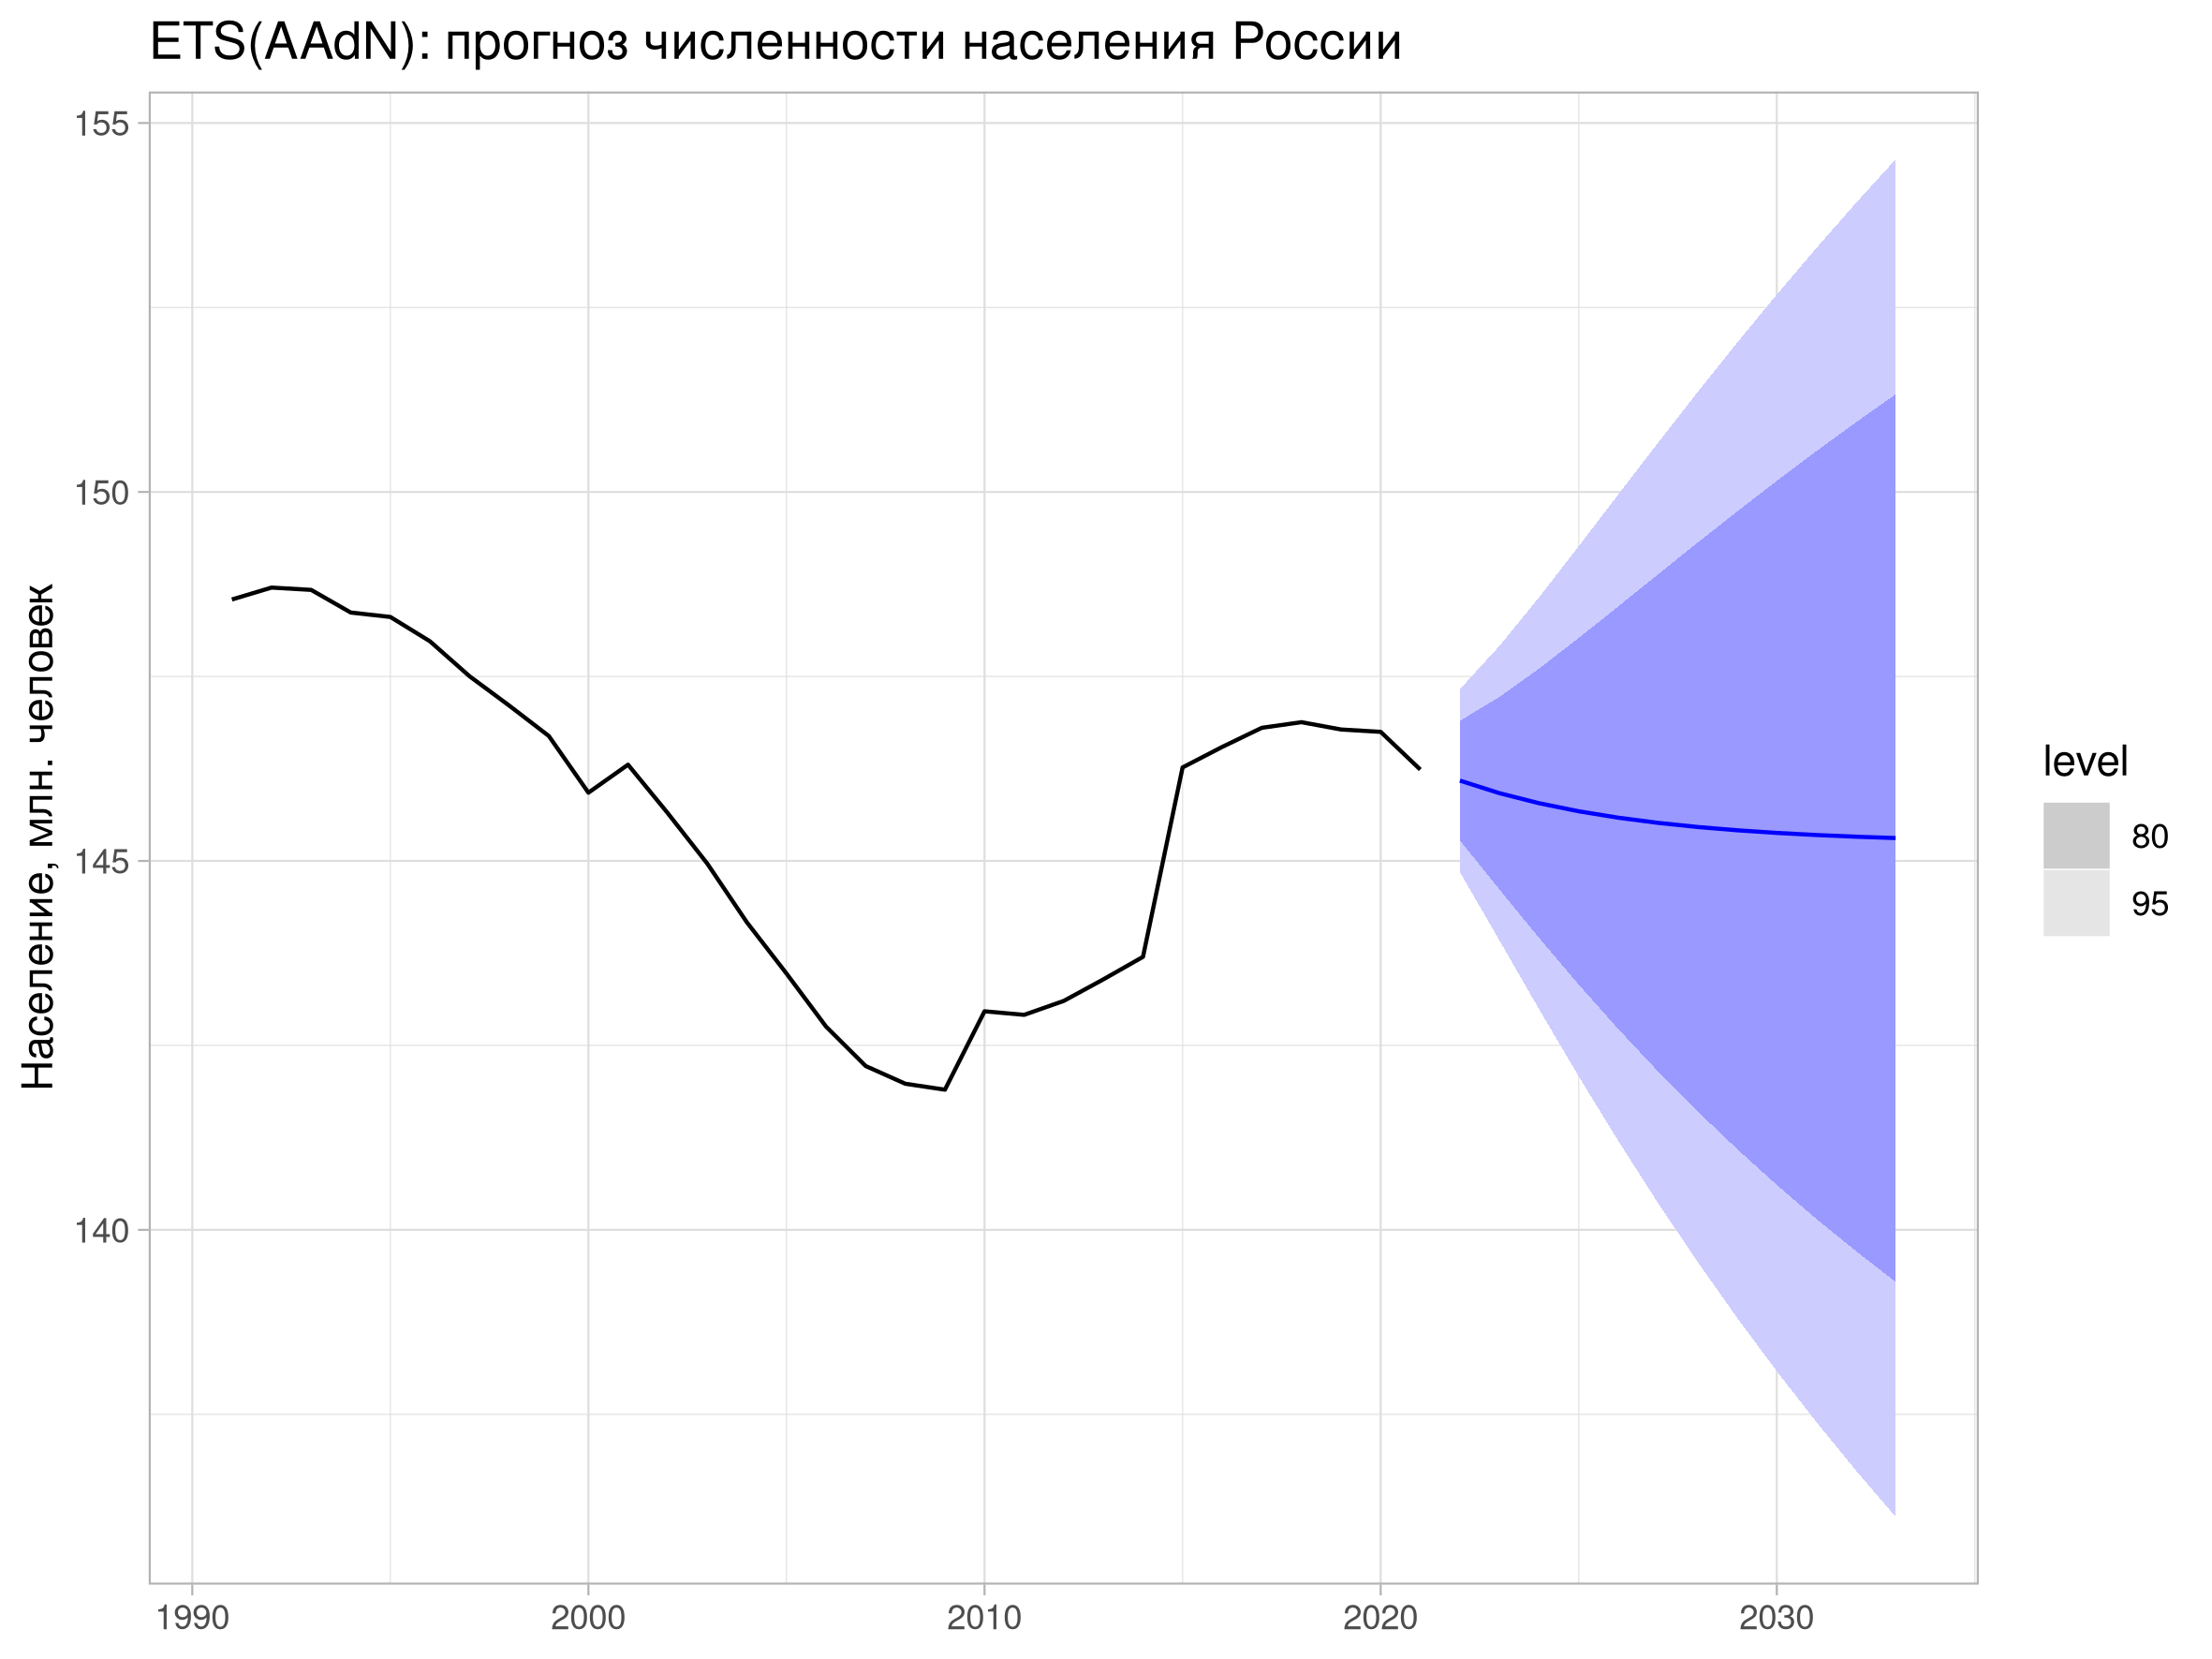
\includegraphics[width=\textwidth]{pictures/om_ts_03-019.png}
  
  % https://www.youtube.com/watch?v=e5WxxvjR9c4
  % я никак не пойму в чём секрет, тренд если есть, то его сразу нет. 

\end{frame}


\begin{frame}
  \frametitle{Прогноз на 1 шаг вперёд}

  \[
      \begin{cases}
        y_t = \ell_{t-1} + \phi b_{t-1} + u_t; \\
       \ell_t = \ell_{t-1} + \phi b_{t-1} + \alpha u_t, \text{ стартовое } \ell_0; \\
       b_t = \phi b_{t-1} + \beta u_t, \text{ стартовое } b_0; \\
       u_t \sim \dN(0;\sigma^2) \text{ и независимы.} \\
       \end{cases}
  \]
  \pause
\[
y_{T+1} = \ell_T + \phi b_T + u_{T+1}  
\]
\pause
\[
  (y_{T+1} \mid \mathcal F_T) \sim \dN(\ell_T + \phi b_T; \sigma^2)  
\]

\end{frame}


\begin{frame}
  \frametitle{Прогноз на 2 шага вперёд}

  \[
    \begin{cases}
      y_t = \ell_{t-1} + \phi b_{t-1} + u_t; \\
     \ell_t = \ell_{t-1} + \phi b_{t-1} + \alpha u_t, \text{ стартовое } \ell_0; \\
     b_t = \phi b_{t-1} + \beta u_t, \text{ стартовое } b_0; \\
     u_t \sim \dN(0;\sigma^2) \text{ и независимы.} \\
     \end{cases}
   \]
  \pause
  \begin{multline*}
    y_{T+2} = \ell_{T+1} + \phi b_{T+1} + u_{T+2} = (\ell_T + \phi b_T + \alpha u_{T+1}) +\\
    + \phi(\phi b_T + \beta u_{T+1}) + u_{T+2} 
  \end{multline*}
   \pause
  \[
  (y_{T+2} \mid \mathcal F_T) \sim \dN(\ell_T + (\phi + \phi^2) b_T; \sigma^2((\alpha + \phi \beta)^2 + 1))
  \]
  
\end{frame}



\begin{frame}{ETS(AAdN): итоги}

  \begin{itemize}[<+->]
    \item На малом горизонте прогнозирования \alert{тренд есть}. 
    \item На большом горизонте прогнозирования \alert{тренда нет}.  
    \item \alert{Один} дополнительный параметр. 
    \item Можно получить ETS(AAdA) модель \alert{с сезонностью}. 
  \end{itemize}
\end{frame}

